\section{Introduction}

\begin{frame}{Lightweight Cryptography}
    \begin{block}{Lightweight Cryptography}
        \begin{itemize}
            \item To implement the ciphers in constrained environments the lightweight ciphers were introduced.
            \item This means a trade off between security and efficiency, but not always.
            \item An effective implementation is PRIDE cipher which do not compromise security for efficiency.
        \end{itemize}
    \end{block}
    
\end{frame}

\begin{frame}{Cipher PRIDE}
\begin{block}{PRIDE}
        \begin{itemize}
            \item PRIDE is a lightweight block cipher introduced in CRYPTO 2014 by Albrecht et al.
            \item The block size and key size are 64-bit and 128-bit respectively and has 20-rounds using SPN implementation.
            \item PRIDE is Software-oriented for widely-used embedded microprocessors.
        \end{itemize}
    \end{block}
    \begin{figure}
        \centering
        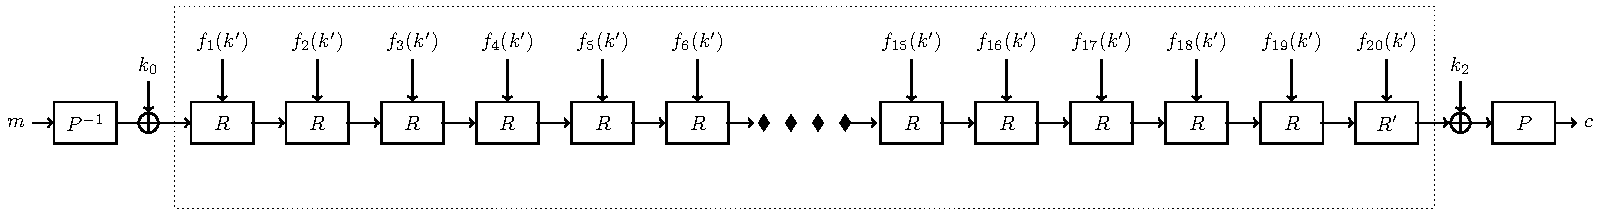
\includegraphics[width=11.5cm]{structure}
        \caption{Overall Structure of PRIDE}
        \label{fig:1}
    \end{figure}
\end{frame}